\documentclass[a4paper]{article}

\usepackage[english]{babel}
\usepackage[utf8]{inputenc}
\usepackage{csquotes}
\usepackage{amsmath, latexsym}
\usepackage{graphicx}
\usepackage{tikz}
\usepackage{listings}
\usepackage{verbatim}
\usepackage{bigints}
\usepackage{float}
\usepackage{titling}
\usepackage[colorinlistoftodos]{todonotes}
\usepackage[style=authoryear,sorting=nty,maxcitenames=1]{biblatex}

\title{Numerical integration of Kirchhoff integral formula and convergence}
\author{}
\date{\today}

\begin{document}
\maketitle

\section*{Abstract}
In this report, we have computed the Kirchhoff integral using the two-point Gaussian quadrature formula and showed fourth-order convergence. The function values are evaluated at quadrature points and emission time without numerical interpolation.

\section*{Kirchhoff integral formula}
The Kirchhoff integral equation for a stationary control surface is given by
\begin{equation}
    \begin{split}
        p'(\mathbf{x}, t) = \frac{1}{4\pi}\int_{S}\Big[  \frac{p'}{r'^{2}}\frac{\partial r'}{\partial n} - \frac{1}{r'}\frac{\partial p'}{\partial n} + \frac{1}{c r'}\frac{\partial r'}{\partial n}\frac{\partial p'}{\partial \tau} \Big]_{\tau} dS.
    \end{split}
\end{equation}
Where, $p'$ is the acoustic pressure satisfying the wave equation outside the control surface \textbf{S}, $c$ is the speed of sound at ambient conditions and $n$ is the normal.
The integrands are evaluated at the emission time $\tau = t - \mathbf{r'}/c$ and $\mathbf{r'}= |\mathbf{x} - \mathbf{y}|$ is the distance between observer and source. 
We compute the integral on a spherical surface. Rewriting the integral using the spherical coordinates, we obtain 
\begin{equation}
    \begin{split}
        p'(r, \theta, \phi,t) =  \frac{1}{4\pi}\int_{0}^{2\pi}\int_{0}^{\pi}\Big[  \frac{p'}{r'^{2}}&\frac{\partial r'}{\partial n} - \frac{1}{r'}\frac{\partial p'}{\partial n} + \frac{1}{c r'}\frac{\partial r'}{\partial n}\frac{\partial p'}{\partial \tau} \Big]_{\tau} R^2\sin\theta d\theta d \phi  
    \end{split} 
\end{equation}
The above integral is numerically computed using the two-point Gaussian quadrature formula
\begin{equation}
    \begin{split}
        p'(r, \theta, \phi,t) =  \frac{1}{4\pi} \sum_{i}^{N_{\theta}}\sum_{j}^{N_{\phi}} \sum_q^{N_q} \Big[  \frac{p'}{r'^{2}}&\frac{\partial r'}{\partial n} - \frac{1}{r'}\frac{\partial p'}{\partial n} + \frac{1}{c r'}\frac{\partial r'}{\partial n}\frac{\partial p'}{\partial \tau} \Big]_{\tau} R^2\sin\theta \Big|_{q} w_q  
    \end{split} 
\end{equation}
\section*{Results}
\begin{figure}!
    \centering
    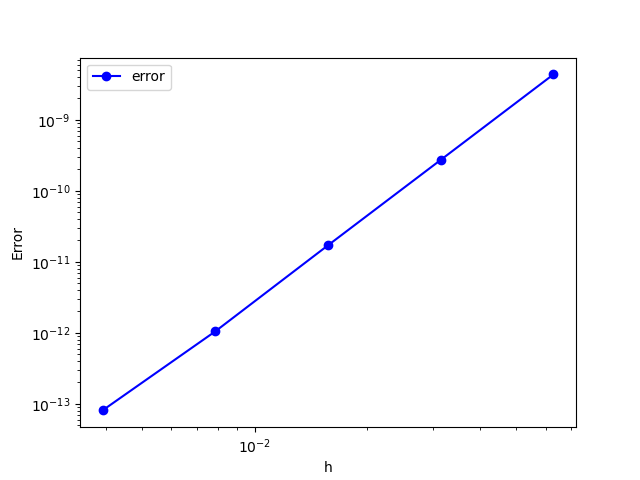
\includegraphics[scale=0.5]{images/convergence.png}
    \caption{We have obtained fourth-order convergence for the Kirchhoff integral computed using the two-point Gaussian quadrature}
\end{figure}
We compute the Kirchhoff integral for a pressure emitted by a monopole source 
$p'(\mathbf{x}, t) = -\frac{1}{4\pi} \frac{  q(t - \frac{r}{c_{0}}) }{r}$. We choose a monopole of strength $q(t) = 2(t - t0)f_{0}^{2}\exp( -f_{0}^2(t - t_{0})^{2})$, 
where $f_{0} = 100$ is the dominant frequency and $t_{0} = \frac{4}{f_{0}}$. Acoustic pressure is computed at observer point ($x_{0}, y_{0}, z_{0}$) $= (3.0, 3.0, 3.0)$ using the Kirchhoff method and compared with the analytical solution. We chose a sphere of radius $R = 1.0$. 
\section*{conclusion}
We have shown the fourth-order convergence of the Kirchhoff integral formula when computed using the two-point Gaussian quadrature formula as expected. We haven't shown the Kirchhoff integral's convergence using the WENO polynomial interpolation.


\end{document}
